\documentclass[varwidth, border=1pt]{standalone}
%\usepackage{subcaption}
\usepackage{subfig}
%\usepackage[labelformat=parens,labelsep=quad, skip=3pt]{caption}
\usepackage{graphicx}
\usepackage[font={small}]{caption}
\begin{document}
\begin{figure}%placeholder1

 \centering
 \subfloat[Original Nucleus Image]{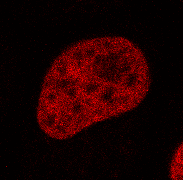
\includegraphics[width = 0.30\textwidth]{fig/OriginalNuc.png}} 
 \quad
 \subfloat[Blurred Nulcleus Image]{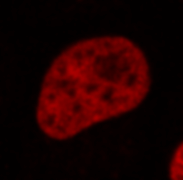
\includegraphics[width = 0.30\textwidth]{fig/BlurredNuc.png}}
 \quad
 \subfloat[Binarized image, after thresholding.]{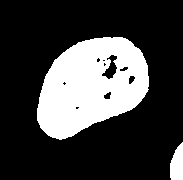
\includegraphics[width = 0.30\textwidth]{fig/ConvertedMask.png}} \\
 \subfloat[Dilated Binary Image]{
\includegraphics[width = 0.30\textwidth]{fig/dilated.png}}
 \quad
 \subfloat[Eroded Binary Image]{
\includegraphics[width = 0.30\textwidth]{fig/eroded.png}}
 \quad
 \subfloat[Subtraction Result, the rim.]{
\includegraphics[width = 0.30\textwidth]{fig/NucRim.png}}
\end{figure}

\end{document}
